\documentclass[11pt, oneside]{article}   	% use "amsart" instead of "article" for AMSLaTeX format
\usepackage{geometry}                		% See geometry.pdf to learn the layout options. There are lots.
\geometry{letterpaper}                   		% ... or a4paper or a5paper or ... 
%\geometry{landscape}                		% Activate for for rotated page geometry
%\usepackage[parfill]{parskip}    		% Activate to begin paragraphs with an empty line rather than an indent
\usepackage{graphicx}				% Use pdf, png, jpg, or eps� with pdflatex; use eps in DVI mode
								% TeX will automatically convert eps --> pdf in pdflatex		
\usepackage{amssymb}
\usepackage{amsmath}
\usepackage{parskip}
\usepackage{color}
\usepackage{hyperref}

\title{Integrate z squared}
%\author{The Author}
%\section{}
%\subsection*{}
\date{}							% Activate to display a given date or no date

\graphicspath{{/Users/telliott_admin/Dropbox/Tex/png/}}
% \begin{center} 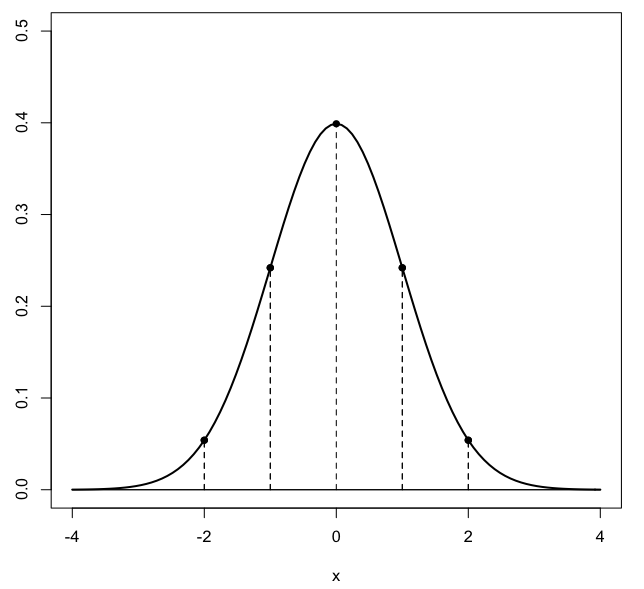
\includegraphics [scale=0.4] {gauss3.png} \end{center}
\begin{document}
\maketitle
\Large

Consider
\[ \int_{\gamma} \frac{z^2}{4-z^2} \ dz \]
where $\gamma = | z + 1 | = 2$.
So the denominator of the function is
\[ \frac{1}{4-z^2} = \frac{1}{(2+z)(2-z)} \]
It has zeroes as $z = \pm \ 2$.  Only the point $z = 2$ is inside our contour.  So if we split this by partial fractions
\[  \frac{1}{(2+z)(2-z)} = \frac{1}{4} \ [ \ \frac{1}{2+z} + \frac{1}{2-z} \ ] \]
so we can rewrite the integral as
\[ I = \int_{\gamma} \frac{z^2}{4} \ [ \ \frac{1}{2+z} + \frac{1}{2-z} \ ] \ dz \]

By Cauchy's Theorem, the first term is zero.  The second one is:
\[ I = \int_{\gamma} \frac{z^2}{4} \ ( \frac{1}{2-z} ) \ dz \]
and the value of $I$ is
\[ I = 2 \pi i f(z_0) \]
where 
\[ f(z_0) = \frac{z^2}{4}  \ \bigg |_{z_0 = 2} = 1 \]
so the integral is just $2 \pi i$.

\end{document}  